\documentclass[a4paper,12pt]{article}
\usepackage{graphicx}
\usepackage{tikz}
\usepackage{setspace}
\usepackage[margin=1in]{geometry}
\usepackage{url}
\begin{document}

\begin{titlepage}
\begin{center}
\vspace*{4cm}

\hrule
\vspace{0.4cm} 
{\LARGE \bfseries Graphs with Identical }\\[1mm]
{\LARGE \bfseries Chromatic Symmetric Functions}\\[0.4cm]
\hrule
\vspace{1.2cm}

\textsc{\Large A Proposal for the}\\[0.2cm]
\textsc{\Large Undergraduate Research Award}\\[2cm]

\begin{minipage}{0.4\textwidth}
\begin{flushleft} \large
\hspace{1cm}\emph{Author:}\\
Keeler M. Russell
\end{flushleft}
\end{minipage}
\begin{minipage}{0.4\textwidth}
\begin{flushright} \large
\emph{Mentor:}\ \ \ \ \ \ \ \ \ \ \ \\
Dr. Jeremy L. Martin
\end{flushright}
\end{minipage}
\vspace{3cm}

\vfill
\includegraphics[scale=0.15]{./figures/kujayhawk.png}\\
\textsc{University of Kansas}\\[0.75cm]
{\large \today}
\end{center}
\end{titlepage}

\begin{spacing}{1}

\section*{\Large Project Description}
\hrule
\vspace{0.4cm}
\subsection*{Summary of Purpose}
All graphs, sets of vertices joined by edges, have an associated chromatic symmetric function $X_G$. This project focuses on whether or not a tree, a particular type of graph, can be reconstructed uniquely from its chromatic symmetric function. This is an open, or unanswered, question in mathematics, defined more fully throughout the course of this proposal.

\subsection*{Background Information}
A \emph{graph} $G$, denoted $G(V, E)$, is a set of vertices $V$ connected by a set of edges $E$. The \emph{order} of a graph is the number of vertices in $V$. A \emph{tree} $T$ is a graph such that any two vertices are connected by a unique \emph{simple path}, a sequence of distinct vertices such that each vertex is connected to the next in the sequence by a single edge. An excellent entry-level introduction to graph theory is \cite{walkthroughcombinatorics}.

We say that two graphs are \emph{isomorphic} if they are structurally identical.  Also, an \emph{invariant} is a property of a graph $G$ that depends only on the structure of the $G$, and not on a particular representation or drawing of $G$. For example, the number of vertices in a graph or number of edges in a graph are simple invariants. Isomorphic graphs, since they are structurally identical, must have the same values for their invariants. However, note that the reverse is not true in general: two non-isomorphic graphs can have the same values for invariants. For example, consider Figure 1: both graphs have the same number of vertices and edges, yet they are clearly unique structurally. A \emph{complete invariant} is one that is unique to an isomorphic graph; that is, only that graph and no others can have that value for the invariant, thus enabling reconstruction of that graph from its invariant.

A \emph{proper coloring} is an assignment of colors to the vertices of a graph such that no two adjacent vertices (vertices which share an edge) share a color. To count the proper colorings of a graph $G$, we use the \emph{chromatic polynomial} $\chi_G(k)$, which counts the number of proper colorings of $G$ given at most $k$ colors. This is another type of invariant. For any tree $T$, $\chi_T(k) = k(k - 1)^{n - 1}$, where $n$ is the number of vertices in the tree. Clearly the chromatic polynomial is useless in distinguishing trees because it gives the same information regardless of the structure of the tree. Building on the chromatic polynomial, Richard Stanley introduced yet another invariant, the \emph{chromatic symmetric function} $X_G$, as a symmetric function generalization of the chromatic polynomial \cite{csfstanley}. The chromatic symmetric function $X_G$ of a graph G is an ordinary generating function which counts, for each integer partition $\lambda\vdash n$, the number of proper colorings that exist using the color $i$ $\lambda_i$ times. For example, in Figure 1, the term $4m_{2,2,1}$ in $X_G$ indicates that there are 4 ways to color two vertices one color, two other vertices a second color, and one final vertex a third color. A standard reference for symmetric functions is \cite{enumerative}. For reference, we denote the chromatic symmetric function of a general graph $G$ is denoted as $X_G$, that of a tree $T$ as $X_T$, and occasionally abbreviate `chromatic symmetric function' as `CSF'.

\subsection*{Research Context}
Here, we may state the overall research question concretely: is $X_T$ a complete isomorphism invariant for trees? That is, does $X_T$ determine a tree's structure up to isomorphism? Or, equivalently, is it possible for any two non-isomorphic trees to have the same $X_T$?

Firstly, it \emph{is} possible for two unique graphs to have the same $X_G$, so it is not a complete isomorphsm invariant for graphs in general (see Figure 1). However, it is unknown whether $X_T$ is a complete isomorphism invariant for trees, which is the question this research aims to tackle. For trees with 23 or less vertices, this question has been answered affirmatively by Li-Yang Tan \cite{tantrees}. Through exhaustive computation, Tan showed that no trees of 23 vertices or less have the same $X_T$.

Additionally, Dr. Martin, et. al. have shown that certain important graph invariants can be recovered from $X_G$ of graphs in general and that for certain classes of trees, $X_T$ distinguishes them up to isomorphism \cite{distinguishtrees}. This is the state of the art for the chromatic symmetric function.

\begin{figure}[t]
\begin{center}
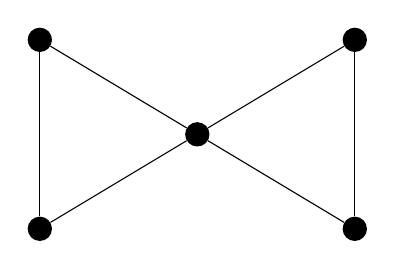
\begin{tikzpicture}
  [scale=.4,auto=left,every node/.style={circle,fill=black,scale=0.5}]
  \node (n1) at (0,0)  {1};
  \node (n2) at (0,6)  {2};
  \node (n3) at (5,3)  {3};
  \node (n4) at (10,6)  {4};
  \node (n5) at (10,0)  {5};

  \foreach \from/\to in {n1/n2,n1/n3,n2/n3,n3/n4,n3/n5,n4/n5}
    \draw (\from) -- (\to);
\end{tikzpicture}
\hspace{1cm}
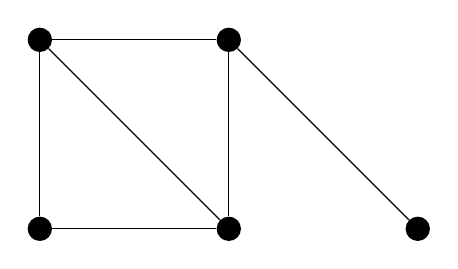
\begin{tikzpicture}
  [scale=.4,auto=left,every node/.style={circle,fill=black,scale=0.5}]
  \node (n1) at (0,0)  {1};
  \node (n2) at (0,6)  {2};
  \node (n3) at (6,6)  {3};
  \node (n4) at (6,0)  {4};
  \node (n5) at (12,0)  {5};

  \foreach \from/\to in {n1/n2,n1/n4,n2/n3,n2/n4,n3/n4,n3/n5}
    \draw (\from) -- (\to);
\end{tikzpicture}
\caption{Two graphs $G$ and $H$ with the same chromatic symmetric function. In this case, $X_G = X_H = 120m_{1,1,1,1,1} + 24m_{2,1,1,1} + 4m_{2,2,1}$.}
\end{center}
\end{figure}

\subsection*{Significance}
This proposal primarily focuses on pure math, an area of research that can be difficult to justify given its lack of direct, real-world significance at conception; the application to the real world often comes later. However, graphs (and especially trees), are utilized to incredible effect in the domain of computer science. Many efficient algorithms and data structures rely heavily on trees as their backbone. I wish to push the frontier of what is known about the chromatic symmetric function of a tree beyond the current state of the art, potentially discerning an answer to Stanley's open question of whether $X_T$ is a complete isomorphism invariant for trees.

\subsection*{Aim of Research}
The first goal is computationally determine whether trees of greater than 23 vertices have the same $X_T$. If this is accomplished, a pair of trees forming a counterexample for the open quesiton given above may be found, and this pair can be analyzed to determine exactly \emph{why} they each have different $X_T$. If such a counterexample is not found, then at the very least the boundary of 23 vertices will have been breached, and the code that I will write for these computations can be made freely available online for future research.

The second goal is purely mathematical: to construct an infinite family of pairs of graphs $(G_0, H_0),\ (G_1, H_1),\ (G_2, H_2),\ \ldots$ for which $X(G_i)$ is identical to $X(H_i)$ for all natural numbers $i$. Stanley, in his original paper introducing $X_G$, presented a pair of graphs which have the same $X_G$, one which looks like a bowtie, the other something like a kite (see Figure 1). By `gluing' copies of these graphs together in a clever way, a method could be provided for constructing an infinite number of graphs with the same chromatic symmetric function. This resembles Gordon and Eisenstat's construction of an infinite family of non-isomorphic `caterpillar' trees with identical subtree data \cite{caterpillarfamily}. Although it would not answer the open question for trees, it would represent an opposing line of inquiry which examines \emph{why} this infinite family has pairs of graphs with the same $X_G$. This could provide insight into what sort of qualities make one graph's $X_G$ differ from another's.

The third, most abstract, and most difficult goal is to treat the chromatic symmetric function as a linear transformation on the vector space of graphs of order $n$ to the vector space of symmetric functions homogeneous of degree $n$. This transformation must have a \emph{kernel} or \emph{nullspace}, a set that contains any of the transformations that result in $0$, since the dimension of the vector space of graphs of order $n$ is much larger than the dimension of the vector space of symmetric functions of degree $n$. The next question to ask would be, "What kind of things exist in this kernel?" Given two graphs $G$ and $H$ of the same order, if $X_G = X_H$ then the formal linear combination $G - H$ is in the kernel. By understanding the kernel of this transformation, it may be possible to gain new insight into the open question of the chromatic symmetric functions of trees. Note that if a tree can be found in the kernel, then two trees share the same CSF, thus answering the question.

\subsection*{Methods}
The first step is to develop a program that generates all non-isomorphic trees on $n$ vertices, then check to make sure that none of them have the same $X_T$. My primary tool in this investigation will be \emph{Sage}, an open-source mathematics software package \cite{sagemath}. For graphs in general, the isomorphism problem becomes infeasible: the number of graphs on $n$ vertices grows exponentially, and a fast algorithm for this process is not known. However, for trees, there exist efficient algorithms for enumerating all trees on $n$ vertices \cite{generatefreetrees} and for checking for isomorphism between two trees \cite{Buss97alogtimealgorithms}. To compute $X_T$ for a given tree T, Stanley gives a formula in \cite{csfstanley} which can serve as the basis for the code.

Constructing an infinite family of trees with identical $X_T$ involves more intuition than programming. Dr. Martin has confirmed this goal's feasibility. I can investigate Stanley's original paper on the chromatic symmetric function further for insight into this problem. Additionally, Dr. Martin's own work serves as an excellent reference for the combinatorial interpretation of the coefficients of $X_G$. With some effort and fact-checking using Sage, I should be able to construct such a family.

The third and final goal is certainly nebulous. At the present time, I believe it is beyond my skill level, and Dr. Martin is not sure whether the approach will turn up anything useful, but that is exactly what makes the research so exciting! In the process of completing the first and second goals of this project, I am confident that I will pick up enough intuition about the chromatic symmetric function to make a reasonable stab at this problem. It is a more generalized version of the second goal, and so the same methods as above will apply.

\section*{\Large Significance to Me}
\hrule
\vspace{0.4cm}
First and foremost, this project is exciting for me. I have already begun to delve in without the grant, and will continue to delve further if not awarded the grant. I plan on continuing my education by acquiring a masters degree, with Computer Science and Mathematics as my two primary choices. As such, I feel that this project is an excellent preparation for graduate study, allowing me to try pushing against the limits of human knowledge in these fields simultaneously before even reaching graduate school.

I would love to see my research published, as I am sure any undergraduate would. More likely, though, I would present at a conference. Dr Martin informed me that many mathematics conferences love to see undergraduate efforts presented. In fact, he mentioned one in particular, the MAA (Mathematical Association of America) conference in San Diego, CA during January 2013. If I planned to present at this conference, that would allow me approximately a year to conduct my investigation.

\section*{\Large My Qualifications}
\hrule
\vspace{0.4cm}
This proposal requires knowledge of computing techniques to develop a correct and efficient algorithm for generating trees and checking their chromatic symmetric functions against one another. A brute force algorithm is out of the question, as such an anlgorithm would be entirely unfeasible given the sheer number of trees it would have to grind through. I feel that I am up to the task for several reasons: for one, I am a Computer Engineering student, and have formal training in algorithm development and analysis. Secondly, I make a living as a programmer working for Garmin on embedded GPS device code, meaning that I have programmed nearly every day for several years. Finally, I was awarded the Eta Kappa Nu Underclassman Achievemnet Award for being the top student in Programming II.

Additionally, during the summer of 2010, just after my freshman semester, I participated in the Honors Research Development Program, drafting a thesis with Dr. Martin. My current proposal is based on the work I completed during that summer, including reading research papers, learning elementary graph theory, and drafting academic papers using \LaTeX. Dr. Martin, however, became busy with classes and several graduate students soon afterward, and I had just started working for Garmin and researching briefly with the Bioinformatics and Computational Life Sciences Laboratory on West Campus. Consequently, the project fell by the wayside. During the interim since then, I have completed more mathematics courses, making me feel much more prepared to tackle a research project like this. With Dr. Martin on sabbatical this semester supporting my efforts and my greater understanding of the tasks at hand, I feel strongly qualified for this project and this research award.

\end{spacing}

\pagebreak
\bibliographystyle{plain}
\bibliography{references}
\end{document}